
%This thesis addresses that OLAP over large property graph is important but current graph databases process graph OLAP in an overwelmingly inefficient manner, and provides an end-to-end efficient solution for it.

OLAP (On-Line Analytic Processing) is the fundamental to many decision-making applications, like smart business, advertising, and risk management. Being a flexible and semantic rich model for graph structured data, the property graph model has been widely adopted and we have seen emerging Graph database systems supporting this model, like Neo4j \cite{DBLP:conf/oopsla/Webber12}, PGX \cite{DBLP:conf/sc/HongDMLVC15}. However, existing graph database systems do not support efficient OLAP queries. Surprisingly, they do not support view-based query or materialize some ``hot'' intermediate results to serve future queries. Therefore, in this thesis, we study the efficient processing of OLAP queries over property graph data using a materialization approach. 


%----------------------------------------------------------------------
\section{Property Graph Model}
%----------------------------------------------------------------------

We are living in an age with exponential growth of data, and a world that is more and more connected.  With the fast development of Web2.0 and Internet of Things(IoT), numerous connections of various kinds are created every second. As a result, massive amount of data of connected systems is generated at the same time. When a user creates a new post not only a post is created,  a ``creates'' connection between the user and the post is established as well. When the user tags the post with a tag, a ``has tag'' connection is built between the tag and the post. When a bank transfer happens, a ``transfers'' connection between two accounts is created.

Property graph is a widely used model for such systems of various connections. A property graph is made of nodes, edges, and properties. Like general graph data models, nodes represent entities and edges represent relationships. For instance, Figure 1.1 is a simple property graph of from online Q\&A forum named www.StackExchange.com. It shows the connections of users (represented by red nodes) and posts( represented by blue nodes). Each arrow pointing from a user node  to a post node represents a ``User\_onws\_Post'' connection. From the graph, we can clearly know that  one user has created 1 post and the other user has created 2 posts. 

We will use a property graph of www.StackExchange.com throughout this thesis. We will call this graph ``StackExchange graph''. 


\begin {figure}[H]
\centering
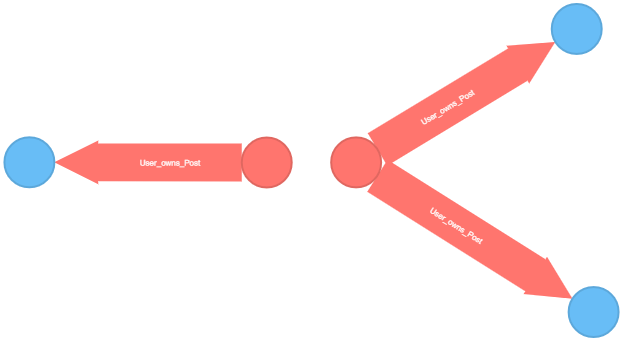
\includegraphics[scale=0.4]{pic/11.png}
\caption{A simple property graph modeling ``users post posts''(data graph).}
\end{figure}


Besides nodes and edges, in property graph nodes and edges can have any number and type of properties. 


For instance, in the exampling property graph, a User node may have properties like the user’s Age, Views, UpVotes etc(listed at the end of the picture). Notice that there is no restriction on what properties a User node can have.  That is, any node or edge could be freely attributed with any type of property. This makes a property graph very flexible in terms of property attribution.
 
Property graph is an informative model as it contains not only nodes and edges, but properties of each individual node and edge as well. 

Meta graph demonstrates graph information on a schema level while data graph refers to the actual graph specific to node and edge level. Figure 1.2 and Figure 1.3 are meta graph and a snapshot of data graph of a property graph on www.stackexchange.com. It contains:

Nodes:	User(in red).
Post(in blue). 
Tag(in green). 
 
Edges: 		User\_owns\_Post. 
Post\_hastag\_Tag.
 
Properties:	User’s View, Post’s Score, Tag’s Tagname etc.

\begin {figure}[H]
\centering
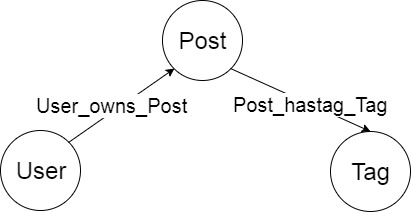
\includegraphics[scale=0.5]{pic/12.jpg}
\caption{Meta graph containing User, Post and Tag.}
\end{figure}
 
\begin {figure}[H]
\centering
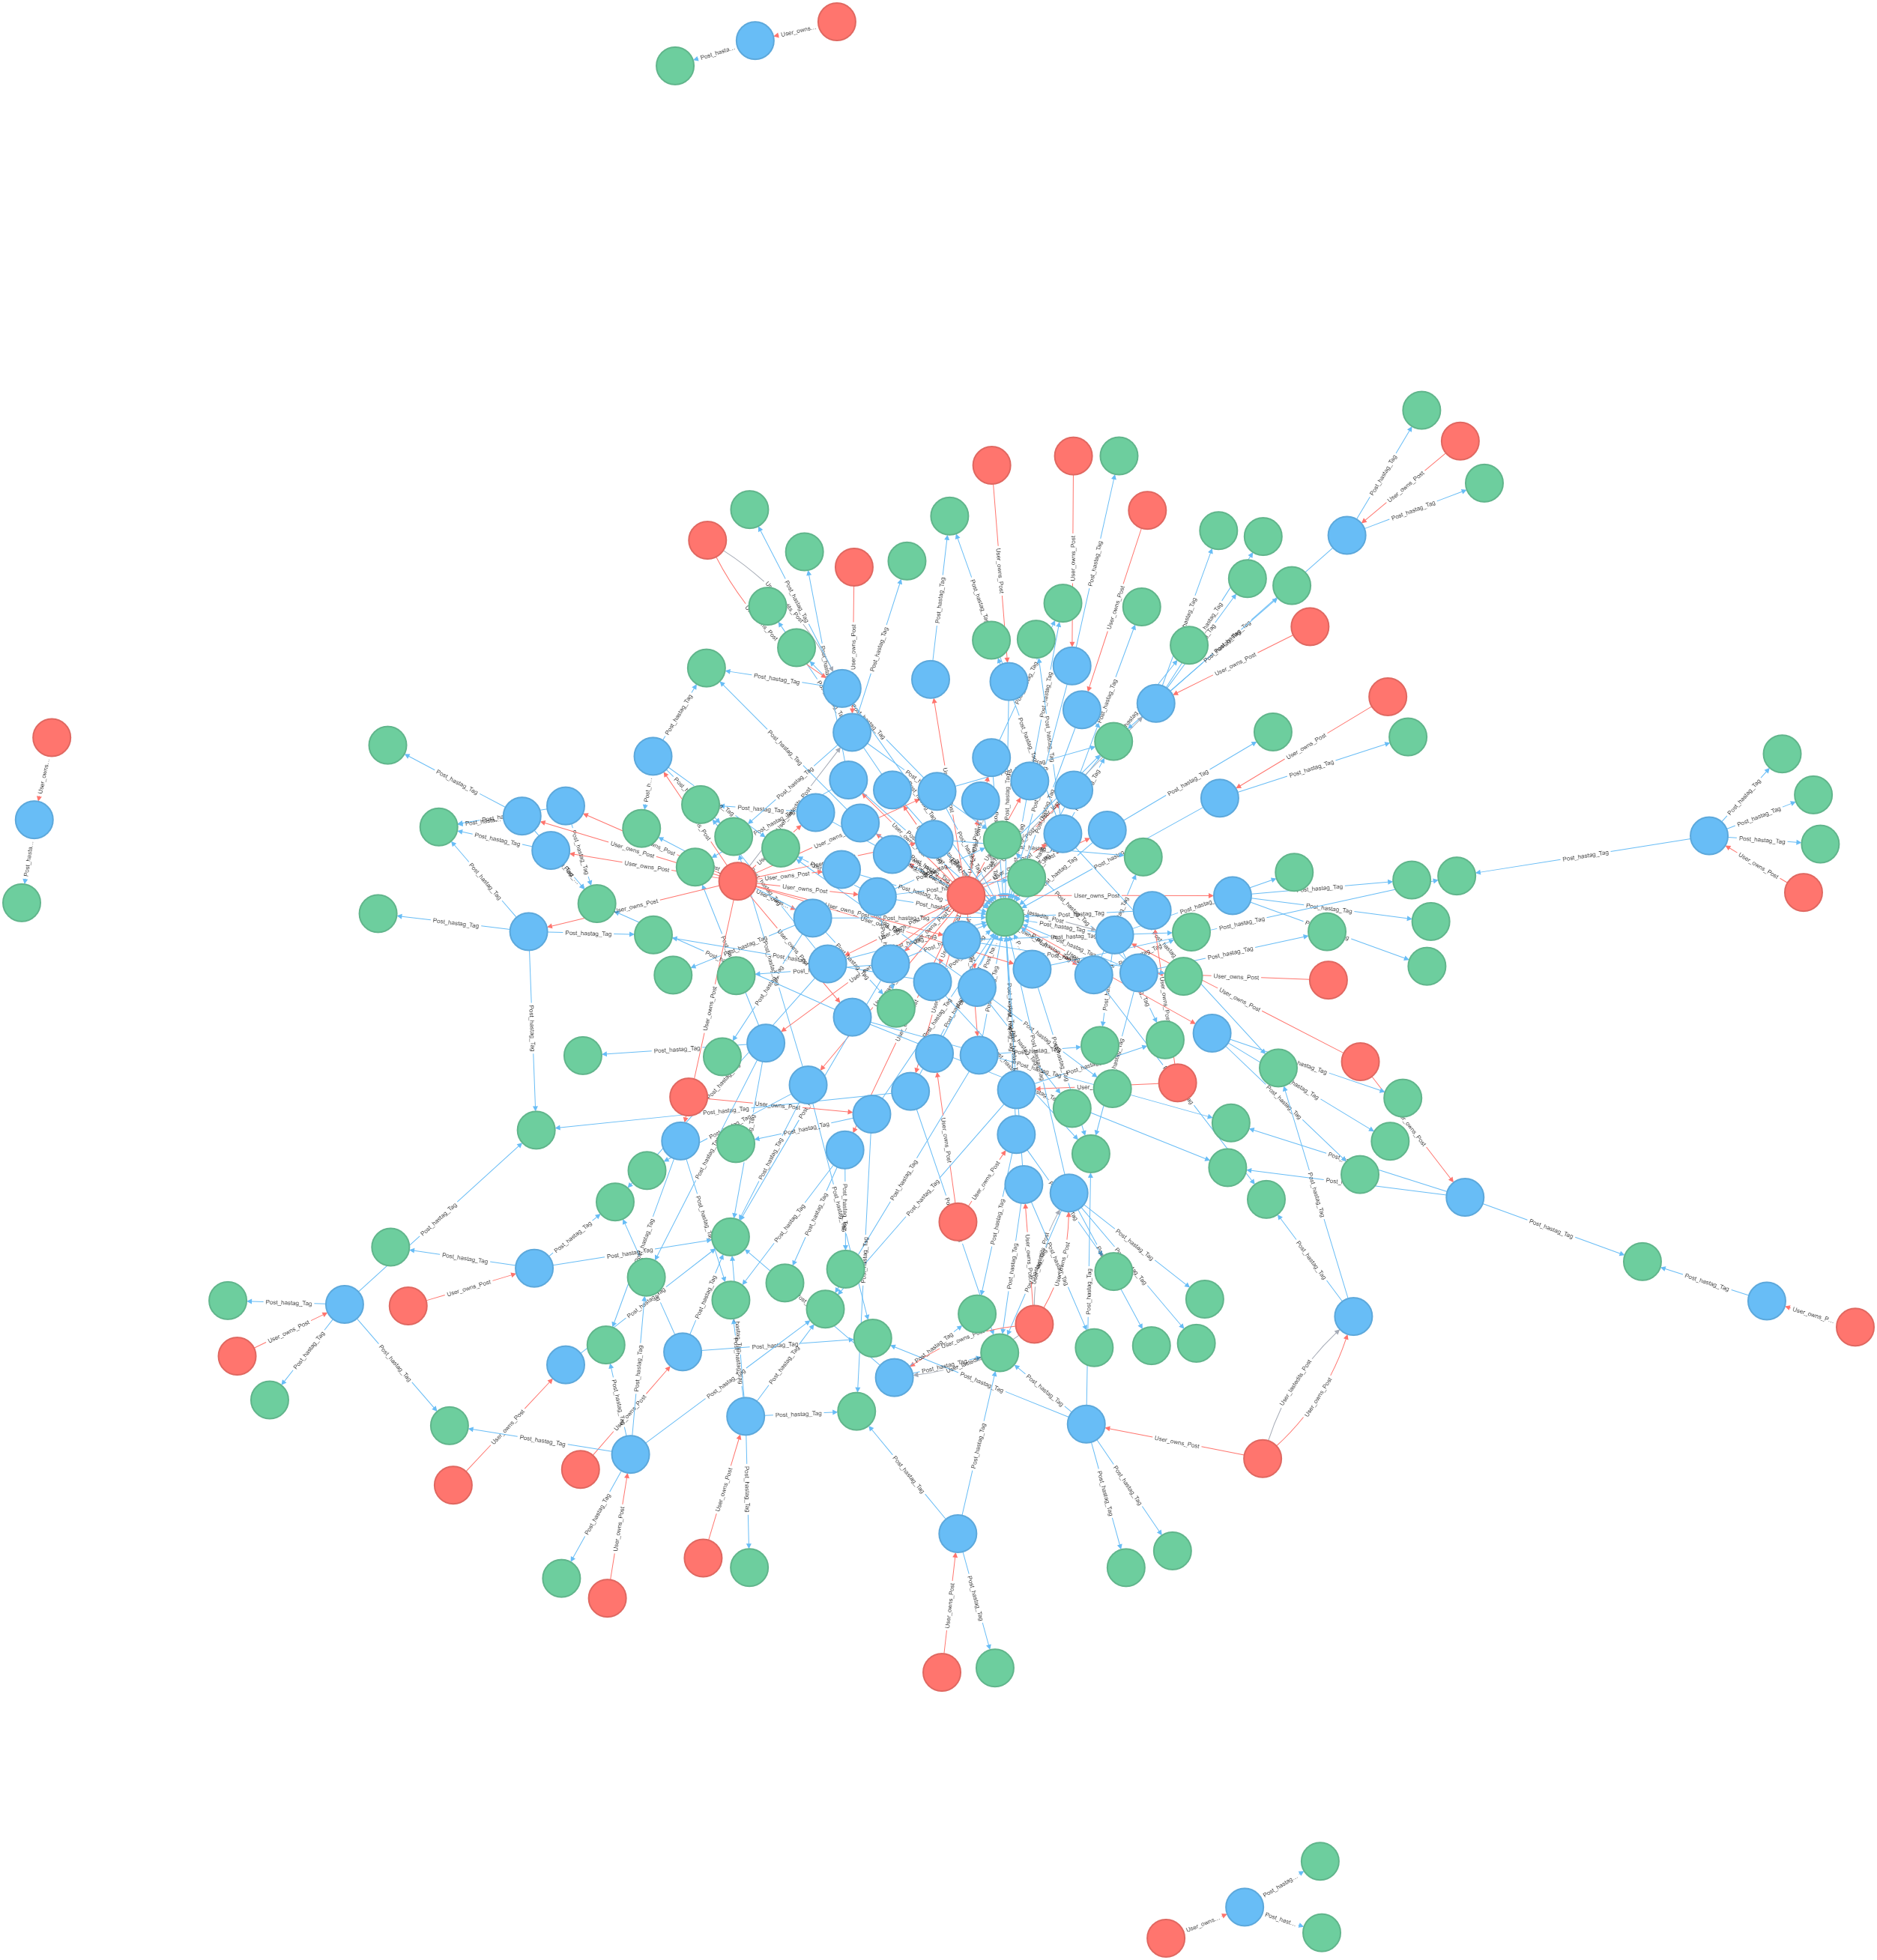
\includegraphics[scale=0.1]{pic/3.png}
\caption{A snapshot of data graph containing User, Post and Tag.}
\end{figure}

%----------------------------------------------------------------------
\section{Graph OLAP}
%----------------------------------------------------------------------


From a property graph we can ask many interesting questions and queries. Among various kinds of queries, OLAP(Online analytical processing) queries play an important role in data analysis. 
 
For instance on ``StackExchange graph'' we may perform OLAP

Query: 		Get average post score grouped by user’s upvotes. 

to see if high upvotes of a user indicate a high-quality post. If the result is shows a significant correlation, we may use the author’s upvotes as a factor to estimate the quality of his or her post when a post is freshly posted and score of the post has not been well voted been yet.


With a property graph dataset on music industry we may ask

Query: 		Get total sum of music purchases by buyers at age 18-25 grouped by music company and month

to evaluate a company's previous strategy in order to increase share of young people's market.

We call such OLAP over graphs ``Graph OLAP''. As a matter of fact, graph OLAP has already been applied in various senerios like business analysis and decision making and it is an interesting research topic in database area.



%----------------------------------------------------------------------
\section{Challenges on Graph OLAP}
%----------------------------------------------------------------------

We know that Graph OLAP is important. However there are many challenges on this topic. One of the most challenging part is efficiency issue. 

From an academic point of view, most of OLAP studies reside in traditional relational data models, whereas studies on efficient graph OLAP are not enough. What's worse, current graph OLAP researches either focus on accelerating graph OLAP over a special subset of property graphs, or focus on general highlevel topics on graph OLAP other than the important issue of query efficiency improvement. 

As a result, current databases do not provide efficent support for graph OLAP, especially when it comes to large datasets. Graph databases are databases that specialize in storage and processing of property graphs. However current graph databases are not satisfactory in terms of OLAP processing efficiency over large property graphs(often with more than millions of nodes and edges). 

	We found that current graph databases like Neo4j process each OLAP query in a naive manner: without using any information of previous queries. In an extreme case, even if we executed a query again and again, execution plan for the query always stays the same and thus execution time does not improve. 

\begin {figure}[H]
\centering
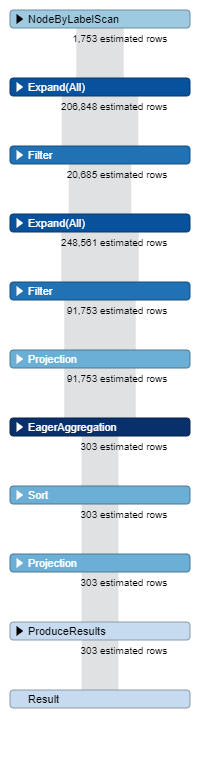
\includegraphics[scale=0.4]{pic/5.png}
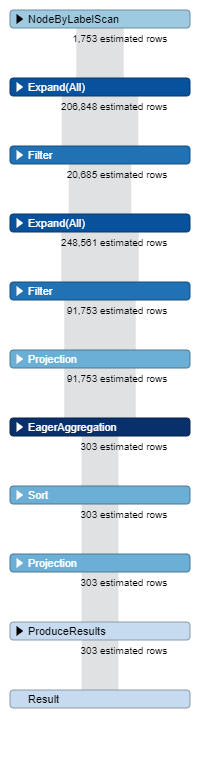
\includegraphics[scale=0.4]{pic/5.png}
\caption{Execution plans of Query \#3 for first time and fifth time.}

\end{figure}

This naive feature of always executing queries regardless of previous queries misses valuable information contained in previous workloads.

For instance, the above exampling OLAP query on StackExchange graph dataset(of roughly 45GB in size) takes Neo4j more than 2 hours to process. It is frustrating for users to wait for 2 hours or even more than a day for the result of one OLAP query as this would undermine interactivity which is one of the most best features of OLAP. Therefore we want to accelerate OLAP processing over large property graphs.

%\begin{center}
%	\begin{tabular}{ | l | l | } 
%		\hline 
%		Query 	& Time	\\ \hline 
%		Query \#1	& \\ \hline
%		Query \#2	& \\ \hline
%		Query \#3	& \\ \hline
%	\end{tabular}
%	\end {center}
	
	


%----------------------------------------------------------------------
\section{Proposed Solution and Contributions}
%----------------------------------------------------------------------
We want to propose a system that supports efficient  OLAP over large property graphs.

 In reality, most OLAP queries are conducted in a real-time manner. As a result, future queries are unknown before they arrive. However in reality a client’s attention tends to reside in several particular structures and properties (closely related with the topics that the client is interested in). Within a specific time range, it is these ``hot'' structures that the client tends to repeatedly view in different dimensions. Therefore previous queries can be used as a good reference for understanding which structures and properties the clients are currently interested in. 
 
For instance, suppose a client just executed the exampling four queries, here is what we can learn from these four previous workload:

Structure-wise: (User)-[creates]-$>$(Post) is frequently queried. We can tell that client is interested in how users create posts. Thus it is reasonable to guess that the user is likely to issue OLAP queries involving (User)-[creates]-$>$(Post) in following queries.
 
Property-wise: User.UpVotes, Post.Score, User.Age, Tag.TagName etc. More specifically, \{User.UpVotes, Post.Score\} and \{User.Age, Tag.TagName\} are frequent combinations. Thus it makes sense to guess that these property combinations are likely to appear together in future queries.
 
Intuitively, if we smartly select frequently queried structures and properties based on previous workload and materialize them, they might be covered in future queries and thus be used to accelerate processing. 
 
A good analogy of this is establishment of materialized views in relational databases and processing queries directly on materialized views. In relational databases, we are allowed to build materialized views on structures and attributes that we are interested in. Hopefully when future queries come, we can faster process them using pre-materialized views. Unfortunately, current graph databases do not support similar operations. 
 
Therefore we propose a system that realizes automatic and smart pre computation and materialization based on finished workload, and utilization of materialized result to facilitate faster future query processing. 
 
There are two most important problems that we need to solve: 
 
One key issue is smart selection of ``materialized views''. We need to select and pre-compute those that are most beneficial for future queries. 
 
Another key issue is how to optimize a better execution plan for answering a future query efficiently using the precomputed materials.

We summurize major contributions of our work is as follows:
\begin{itemize}
\item {We designed an end-to-end system that realizes structure-aware OLAP query processing on graph databases using precomputation based on previous workloads.}

\item We implemented our system on Neo4j.

\item We proposed our algorithm for smart selection of structures and cuboids to be precomputed.
 
\item We suggested different ways for future query processing. We tested their performances and gave explanations on the performance differences.
 
 \end{itemize}

The following contents are organized in this way:
In part 2 we will discuss about related work. We will introduce pre-military knowledge about  OLAP, graph databases, Neo4j; and provide a summary of how existing work solves OLAP queries.
In part 3 we will explain our solution framework and system design in details. 
Part 4 is on experiments. We will talk about experiment design, followed by presentation of experimental results and discussions of results.
Part 5 will talk about opening questions and future work.

